\section{Visualization of Provenance Data}

We characterize the visualization of provenance data based on the level of semantics involved in the collected data~\cite{Gotz2009}, including event, action, sub-task and task. Because low-level events contain little semantics, they are often visualized and analyzed after users finished their tasks in order to gain deeper understanding about their processes rather than to provide near real-time sensemaking support to the users during their tasks. For example, visualization of users' mouse clicks can reveal patterns of application usage~\cite{Matejka2013} and highlight some important usability issues, such as pages where users spent a lot of time and pages where they got lost during the task~\cite{Waterson2002}. User interactions with visual analytics systems can be visually examined to recover their reasoning processes employed in their analysis tasks such as specific findings they found and strategies they used~\cite{Dou2009, Guo2016}. Interaction logs have also been used to predict user performance of basic visualization tasks like visual search~\cite{Brown2014}.

Next, we focus on the visualization of levels with richer semantics. Actions and states
(the visualization results of the actions) are commonly used to show the analysis process. Sub-tasks and tasks are often documented by users in a graphical reasoning process.

\subsection{Visualization of Analysis Process}

\subsubsection{Visual Representation}

\paragraph{Text}
Text is commonly used to describe actions or states, such as names of actions, titles of visited web pages and content of user notes. Text can provide accurate information, but long text makes it difficult for users to understand and recognize. A graphical browser history by Ayers and Stasko~\cite{Ayers1995} shortens web page titles to accommodate more pages in the view. Within a given width, its algorithm preserves complete words at both ends of the title and trims characters in the middle if necessary. Kaasten, Greenberg and Edwards~\cite{Kaasten2001} compare the recognizability of titles between various string sizes for all three truncation methods (text is truncated at the beginning, middle or end of the title). The results show that for medium (60\%) recognition, we need 15--20 letters (depending on
the truncation method) for web sites, and 28--39 letters for
exact pages. For longer text such as user notes, machine learning techniques for text summarization could be beneficial~\cite{Nenkova2012}.

\paragraph{Icon}
Sensemaking actions can be represented by graphical symbols, allowing users to easily distinguish them. They can be used alone to represent the analysis process when the visual result of each action is out of interest (\autoref{fig:lr-action-1}). Alternatively, these icons can be used together with interface states, connecting the one before and the one after an action (\autoref{fig:lr-action-2}).

\begin{figure}[!htb]
\centering
\subcaptionbox{A sequence of icons displaying the analysis process. \is{Gotz2009}\label{fig:lr-action-1}}{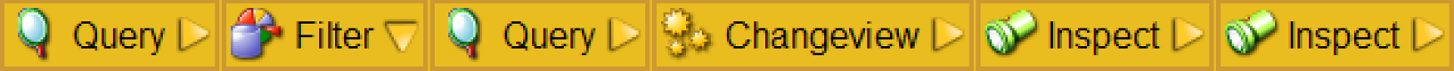
\includegraphics[width=.8\columnwidth]{action-1}}

\vspace{.5\baselineskip}

\subcaptionbox{Iconic actions connecting two visualization states. \is{Ma1999}\label{fig:lr-action-2}}{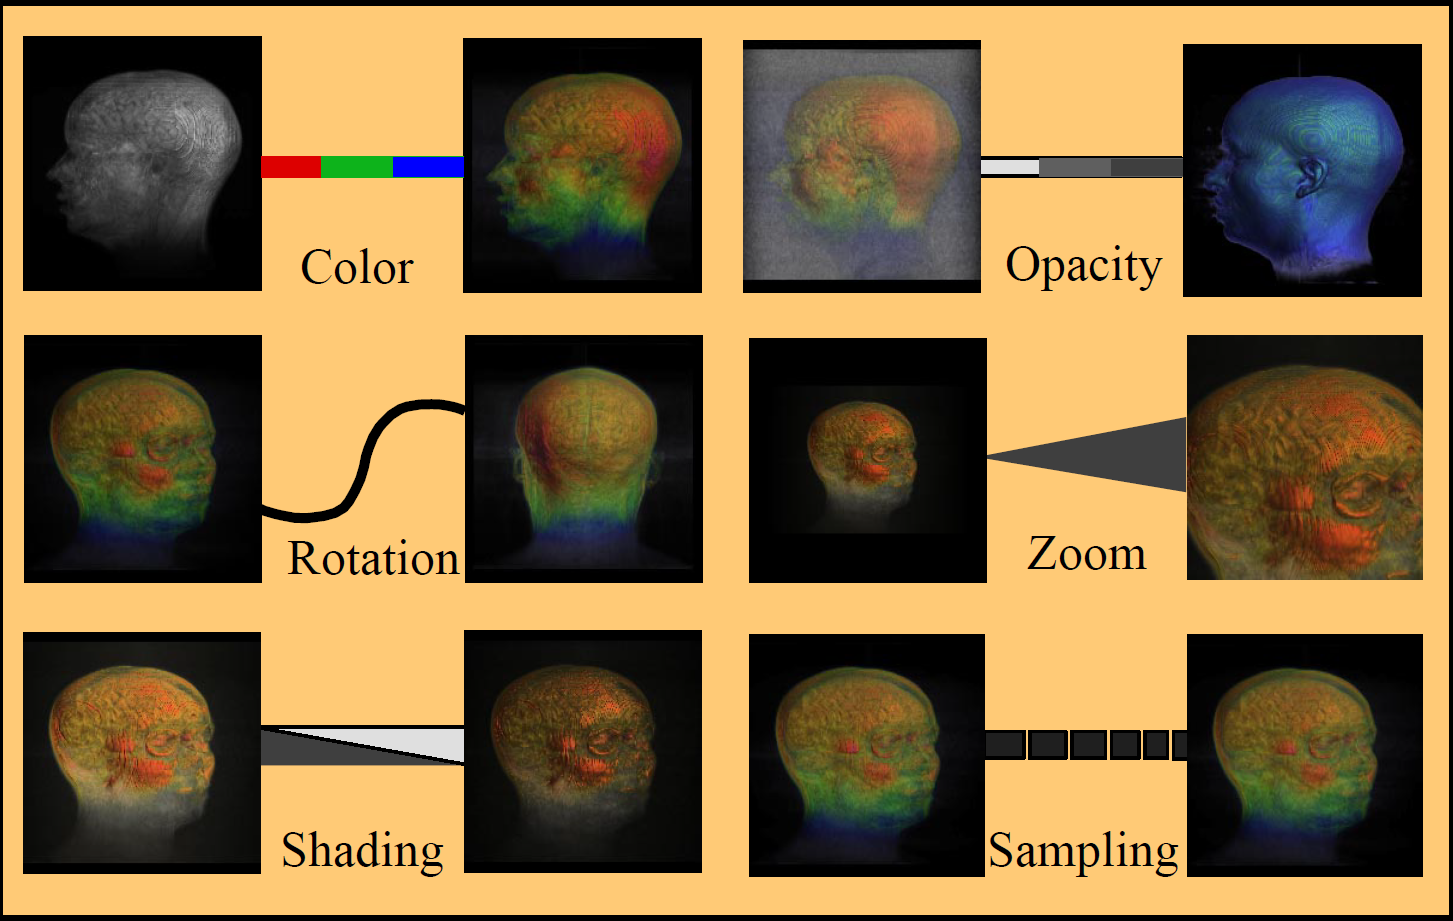
\includegraphics[width=.8\columnwidth]{action-2}}
\caption{Using icons for representing actions.}
\end{figure}


\paragraph{Thumbnail}
Thumbnails are commonly used to represent visualization states, aiding users' recognition of previous ones. One study suggests that a thumbnail size of 96 pixels square could provide 60\% accurate recognition of a visited web site~\cite{Kaasten2001}. For the same accuracy but in recognizing an exact web page, the thumbnail size rises to 144 pixels square. Additional information can be added to a web thumbnail to improve its recognition such as how often the represented page is revisited and whether that page is bookmarked or not~\cite{Cockburn1999}. For visualization thumbnails, visual encodings and parameters that were used to produce the visualization can also be embedded (\autoref{fig:lr-thumbnail-encoding}), providing more provenance information to the users.

\begin{figure}[!htb]
	\centering
	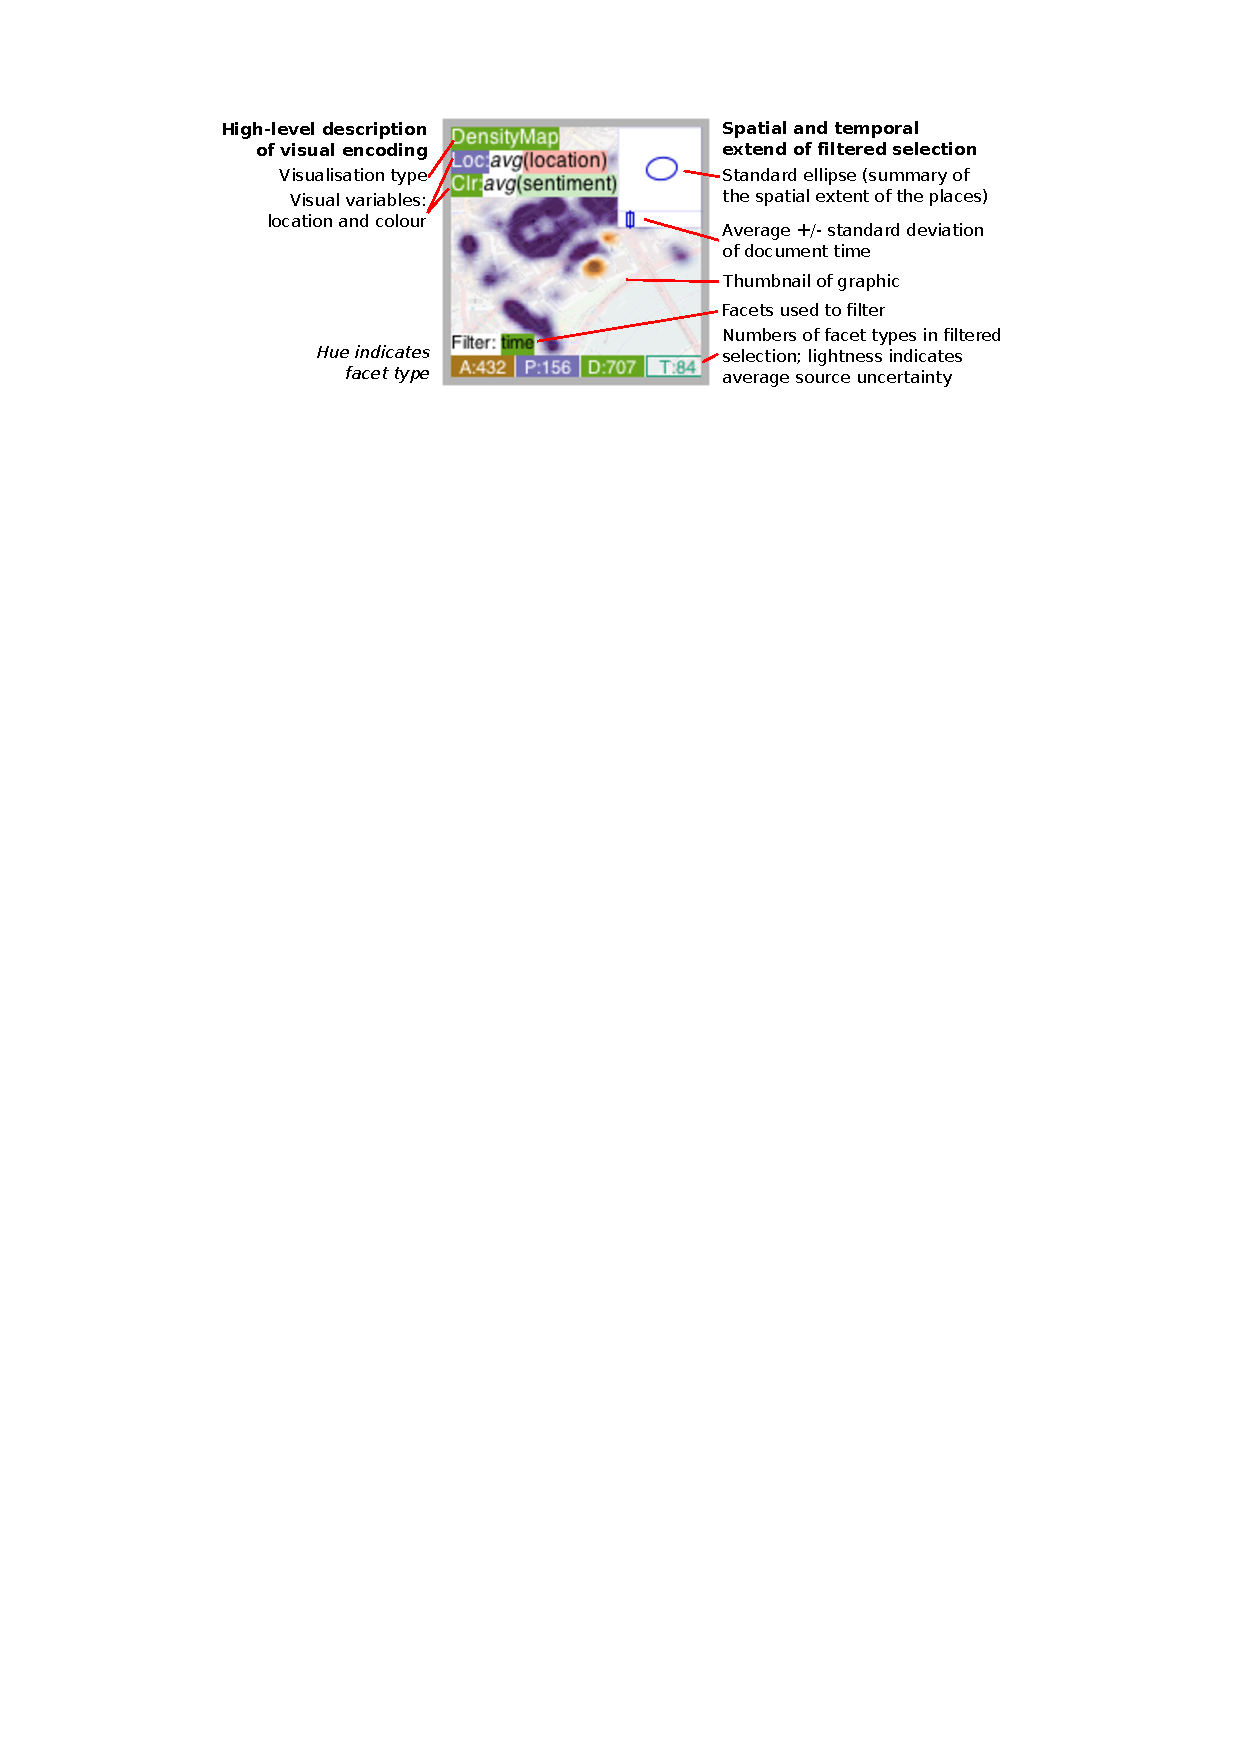
\includegraphics[width=\columnwidth]{thumbnail-encoding}
	\caption{Visualization thumbnails with additional information about any filtering used, the characteristics of the filtered subset of data and the visual encoding. \is{Walker2013}}
	\label{fig:lr-thumbnail-encoding}
\end{figure}

It may be necessary to apply pre- and post-processing adjustments to make the visualization thumbnails more recognizable~\cite{Heer2008}. For example, high-frequency visual elements that are not helpful in a small size such as gridlines and element borders can be removed to prevent their domination in the resulting thumbnail. As a result of down-sampling techniques, colors of data items may be different from them in the original visualization. Therefore, readjusting the color to match its intended value could help users to recognize the visualizations they analyzed in the past.

The default snapshot may also be an imperfect representation of a web page, especially if it contains a lot of text. Teevan~et~al.~\cite{Teevan2009} propose an automatic method to produce a thumbnail improving its recognition. It consists of three components: some salient text at the top-left hand corner, a salient image below the text, and a watermarked logo superimposed at the bottom left hand corner of the image. The salient text contains about 20 first characters of the web page title. The salient image and the branding logo are chosen from the page using machine learning. \autoref{fig:lr-enhanced-thumbnail} shows such a thumbnail.

\begin{figure}[!htb]
	\centering
	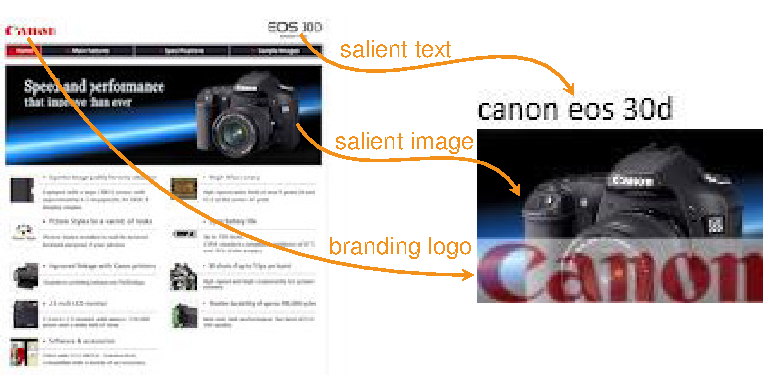
\includegraphics{enhanced-thumbnail}
	\caption{An enhanced web thumbnail (right) as a composite of some salient text, a salient image and a branding logo. \is{Teevan2009}}
	\label{fig:lr-enhanced-thumbnail}
\end{figure}

Besides recognizing previous states, seeing the difference between a state and the one before it is also important in understanding the analysis process. One approach is to highlight the difference between two consecutive states (\autoref{fig:lr-state-2}). The changes may only happen at one small portion of the entire interface. Therefore, showing only that area in both states could help users quickly identify the difference (\autoref{fig:lr-state-3}).

\begin{figure}[!htb]
\centering
\subcaptionbox{Modified items are highlighted with green borders. \is{Klemmer2002}\label{fig:lr-state-2}}[.47\columnwidth]{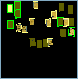
\includegraphics[height=.33\columnwidth]{state-2}} 
\hfill
\subcaptionbox{Changed area is cropped and shown in both  states. \is{Kurlander1988}\label{fig:lr-state-3}}[.47\columnwidth]{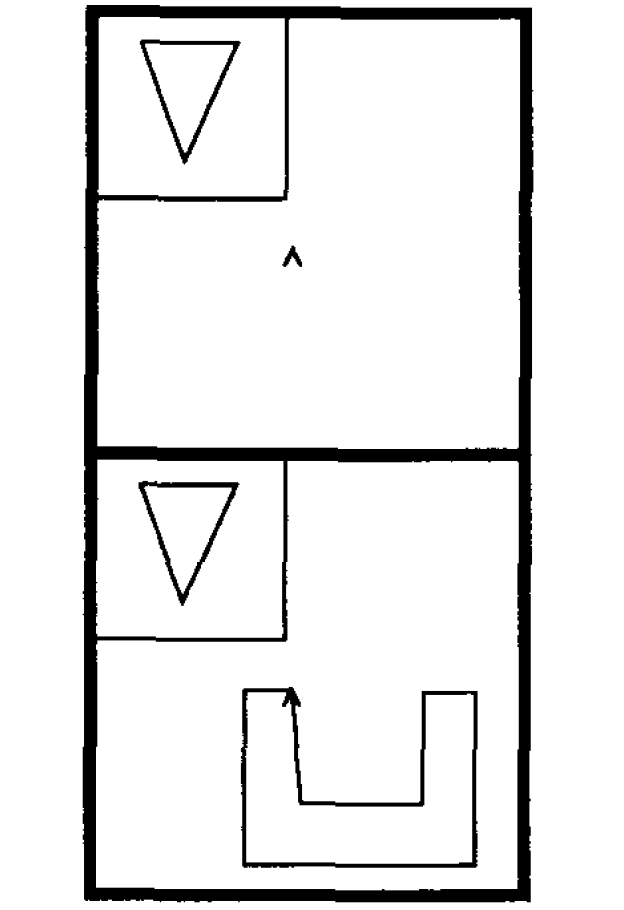
\includegraphics[height=.33\columnwidth]{state-3}}
\caption{Techniques improving recognition of state changes.}
\end{figure}

\subsubsection{Layout}

\paragraph{Linear Layout}
Provenance data usually contains an inherent \emph{time} attribute, recording when an action happened. An approach that emphasizes on the order of completed actions is to show them as a linear sequence of items like a comic strip~\cite{Kurlander1988,Meng1998}. This layout facilitates visual scanning of past actions, allowing users to quickly understand the analysis process. \autoref{fig:lr-comic-strip} shows such a layout.

\begin{figure}[!htb]
	\centering
	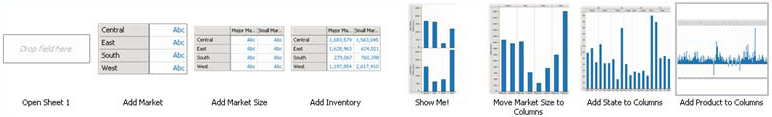
\includegraphics[width=\columnwidth]{comic-strip}
	\caption{Comic strip layout. A sequence of past actions in chronological order. \is{Heer2008}}
	\label{fig:lr-comic-strip}
\end{figure}

If the absolute timestamps of actions are of interest, a continuous timeline~\cite{Derthick2001} is a more suitable layout. Actions are positioned along the time axis at when they happen (\autoref{fig:lr-continuous-timeline-1}) or during which they last (\autoref{fig:lr-continuous-timeline-2}). The time axis can be either horizontal or vertical~\cite{SandboxTimeline2012}. The layout algorithms found in these provenance timelines are quite naive. POLESTAR~\cite{Pioch2006} and the timeline from Jigsaw~\cite{Liu2010} require manual rearrangement of the events from users to solve the overlapping problem. The timeline from nSpace2 Sandbox~\cite{SandboxTimeline2012} shows events at the exact time when they happen without considering possible intersection between of them.

\begin{figure}[!htb]
\centering
\subcaptionbox{Time-point provenance data. User annotations are positioned along a time axis at when their associated events happen. \is{Gotz2006}\label{fig:lr-continuous-timeline-1}}{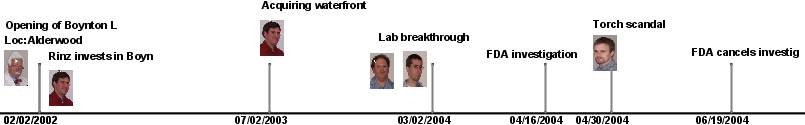
\includegraphics[width=\columnwidth]{continuous-timeline-1}}

\vspace{.5\baselineskip}

\subcaptionbox{Interval provenance data. User actions are shown as horizontal bars a long a time axis covering their durations. \is{Plaisant1999}\label{fig:lr-continuous-timeline-2}}{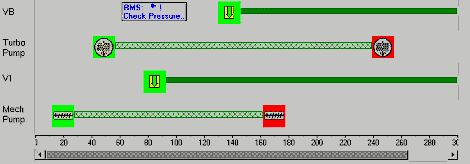
\includegraphics[width=\columnwidth]{continuous-timeline-2}}
\caption{Timeline layout for visualizing the analysis process.}
\end{figure}

Another approach is to use both the horizontal and vertical axes to represent time. BrowseLine~\cite{Hoeber2009} uses the vertical axis for \emph{macro-time} and the horizontal axis for \emph{micro-time}, similar to stem-and-leaf plots. More specifically, a two-dimensional timeline (\autoref{fig:lr-timeline-2d}) is divided into rows, each for a big time-slot, such as one hour. In each row, events happening within that hour are positioned along the horizontal axis without considering their absolute timestamps. This design assumes that users may only remember roughly when events happen, thus absolute positioning in the vertical axis facilitate them in recognizing past events. Moreover, relative positioning in the horizontal axis could help pack more events and prevent overlapping.

\begin{figure}[!htb]
	\centering
	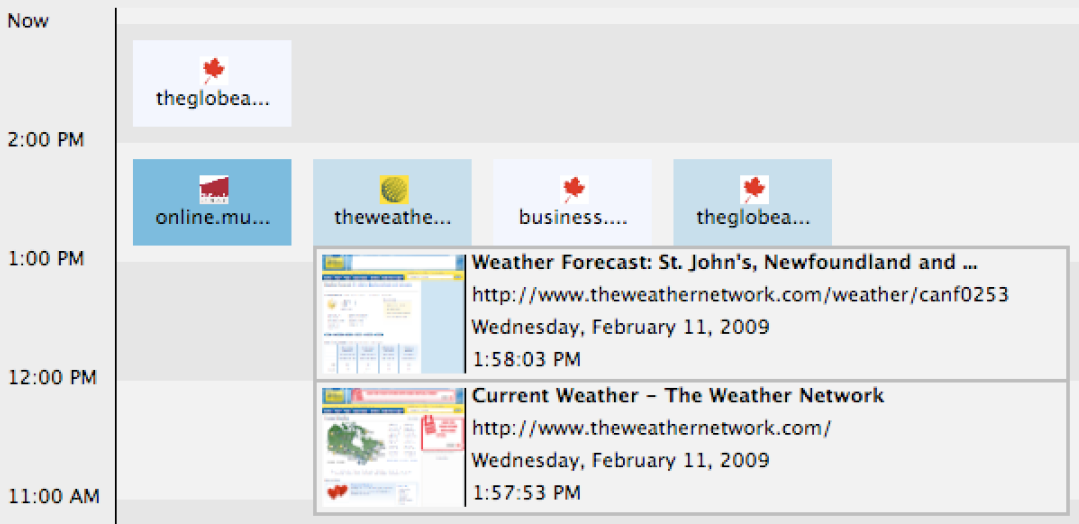
\includegraphics[width=\columnwidth]{timeline-2d}
	\caption{2D timeline. The vertical axis represents macro-time, whereas the horizontal axis represents micro-time. Events within a macro time-slot are positioned in chronological order as a comic strip. \is{Hoeber2009}}
	\label{fig:lr-timeline-2d}
\end{figure}

\paragraph{Branching Layout}
Many sensemaking systems allow users to revisit their past states such as through undo/redo features or backward/forward in web browsers. From a past state, if the user performs a new action, it should be recorded in a new branch forking from that state. This branching history is typically visualized with a tree layout to represent the logic of the analysis process effectively. In such a tree, nodes represent a summary of system states, and edges represent actions that transition the system from one state
to another. Examples can be found in provenance-enabled systems in different fields including scientific visualization~\cite{Ma1999}, information visualization~\cite{Dunne2012}, visual analytics~\cite{Kadivar2009} and browser history~\cite{Ayers1995}. \autoref{fig:lr-tree} shows such a provenance tree.

\begin{figure}[!htb]
	\centering
	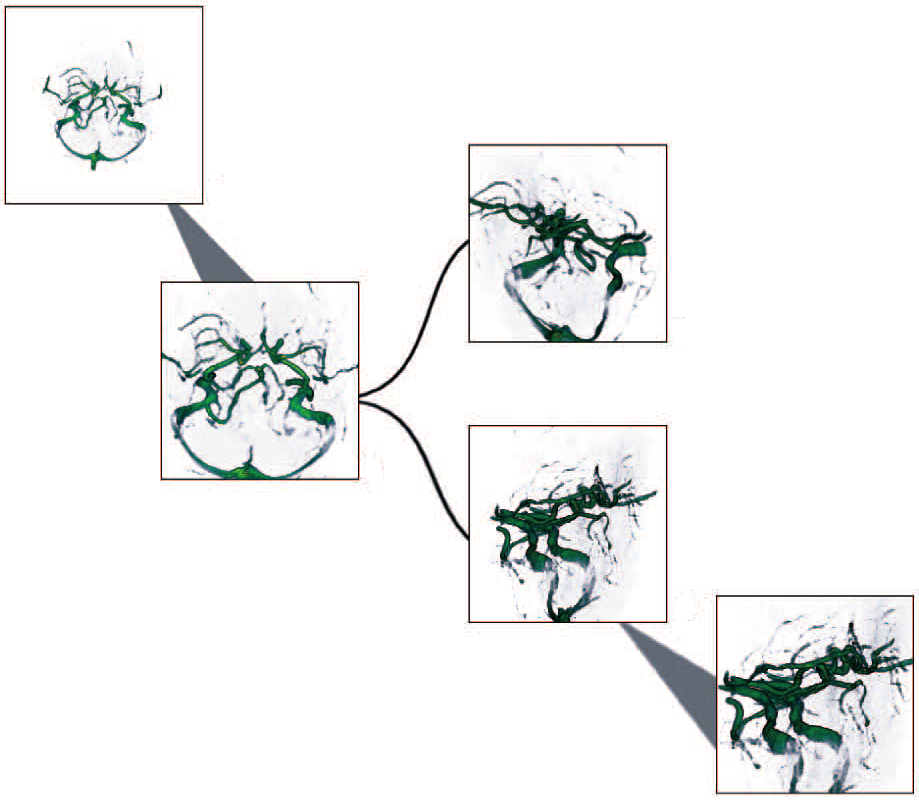
\includegraphics[width=.7\columnwidth]{tree}
	\caption{Tree visualization for branching analysis process. Nodes are thumbnails of past visualization states and links are transforming actions. \is{Jankun-Kelly2007}}
	\label{fig:lr-tree}
\end{figure}

% Time encoding
In a tree layout, the order of actions can be inferred through the direction of edges. Moreover, exact time gap between actions can also be visually encoded into the visualization. VisTrails~\cite{Bavoil2005} color-codes the background of nodes according to their creation time (\autoref{fig:lr-tree-time-1}). Aruvi~\cite{Shrinivasan2008} uses the length of edges to represent the relative time gap between two states (\autoref{fig:lr-tree-time-2}). 

\begin{figure}[!htb]
\centering
\subcaptionbox{Node backgrounds are color coded based on time. \is{UniversityofUtah2012}\label{fig:lr-tree-time-1}}{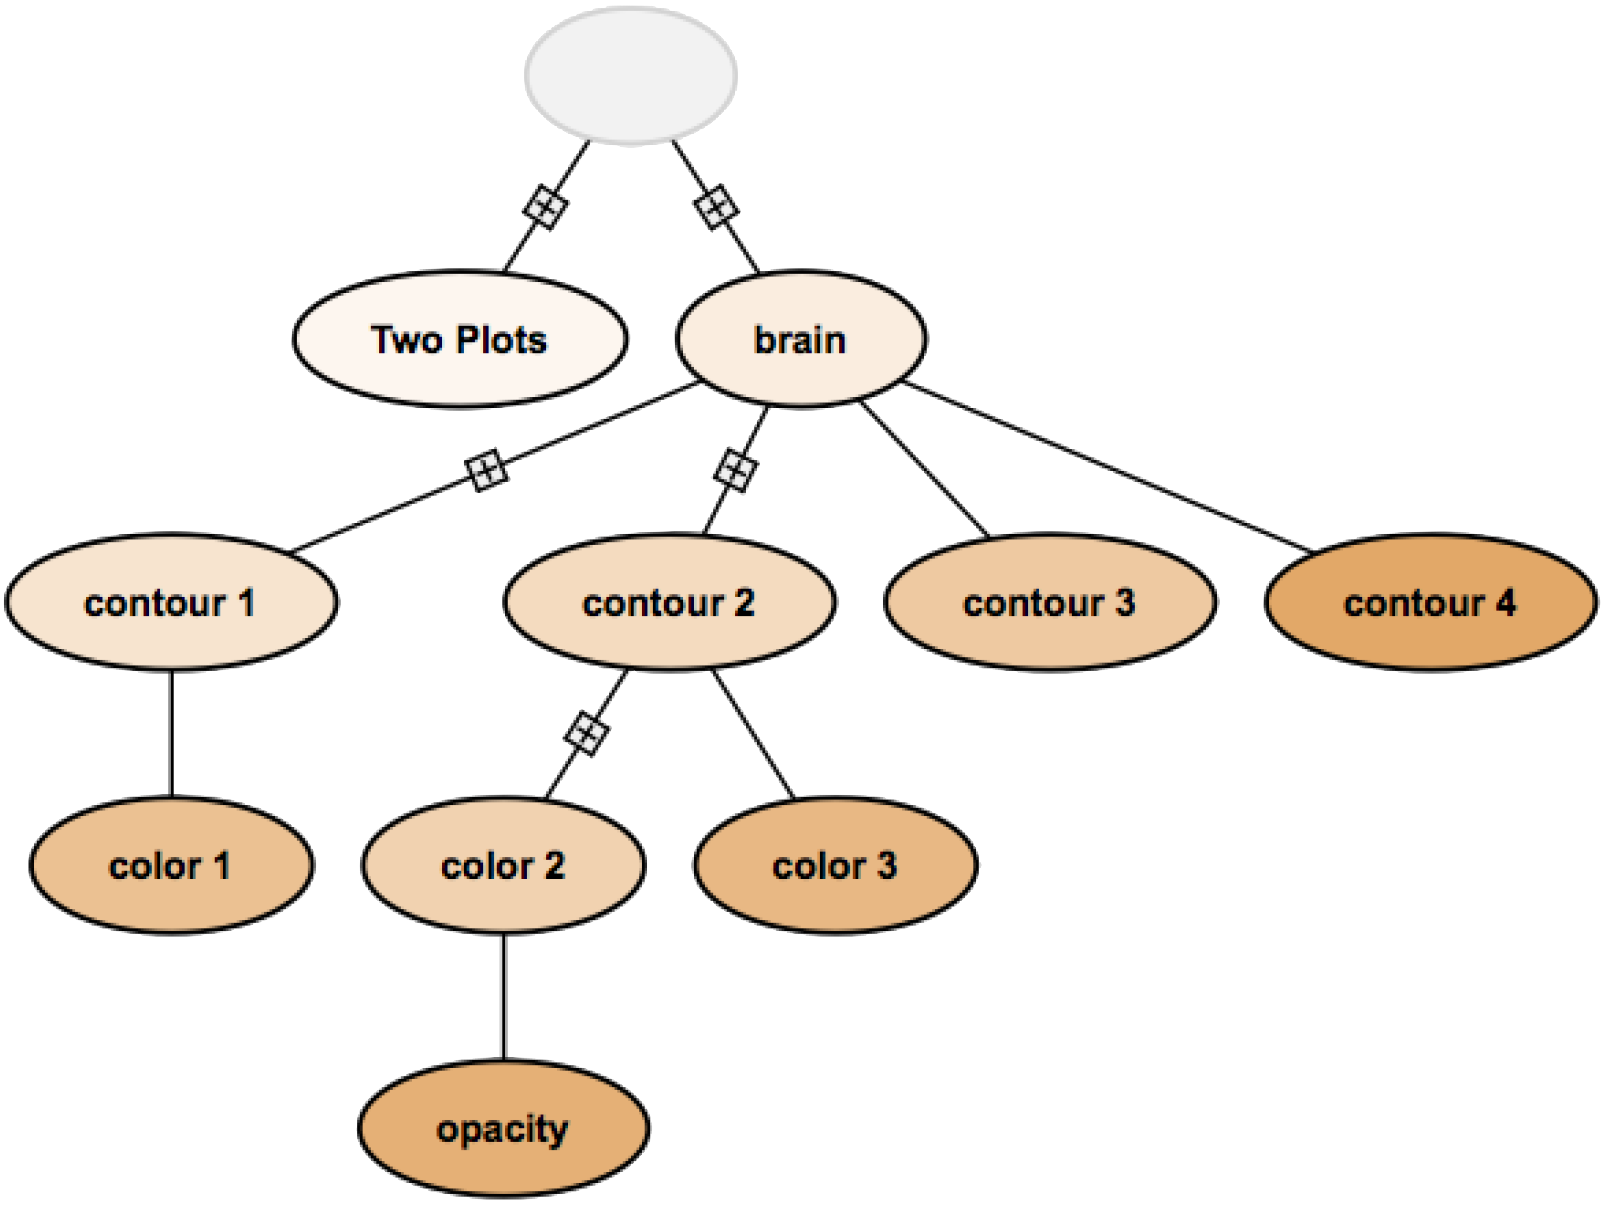
\includegraphics[height=0.21\columnwidth]{tree-time-1}} 
\hfill
\subcaptionbox{The edge length between two nodes represents the interval between them. \is{Shrinivasan2008}\label{fig:lr-tree-time-2}}{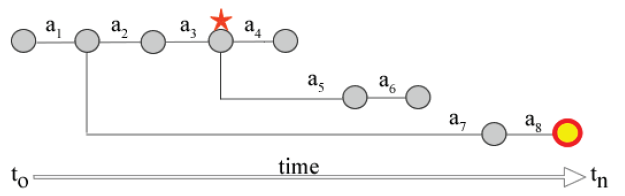
\includegraphics[height=0.21\columnwidth]{tree-time-2}}
\caption{Encoding temporal information into provenance trees.}
\end{figure}

% Other variations
The diagonal arrangement of tree as in~\autoref{fig:lr-tree} may consume a lot of space. One approach is to use only horizontal and vertical edges as in~\autoref{fig:lr-tree-time-2}. Another approach is to display only the path that led to the currently active  visualization~\cite{Klemmer2002}. Other paths can be expanded on demand. \autoref{fig:lr-inline-history-2} shows examples of representations of the active path and the full history.

\begin{figure}[!htb]
\centering
\subcaptionbox{Branched history. The user first performed actions $A$, $B$, $C$, $D$ and $E$, then undone to $D$, $C$ and $B$, then performed new actions $F$ and $G$.  \label{fig:lr-inline-history-1}}{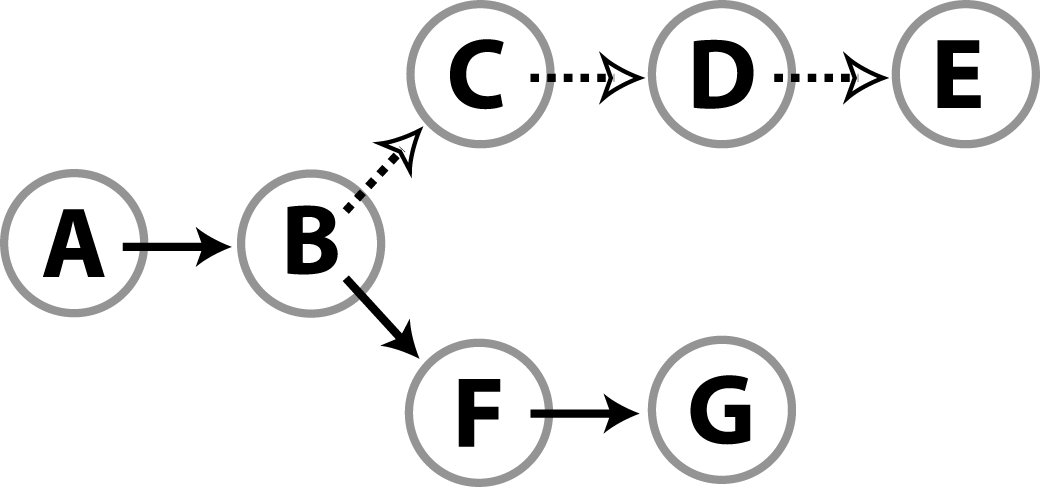
\includegraphics[height=.178\columnwidth]{inline-history-1}}
\hfill
\subcaptionbox{Inline branching history representation. Top: displaying the current path. Bottom: displaying the full history; actions not part of the current path are placed between brackets. \label{fig:lr-inline-history-2}}{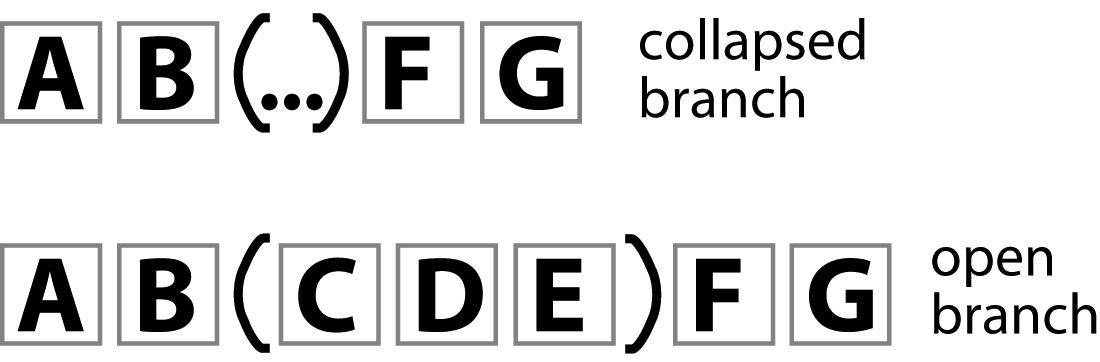
\includegraphics[height=.188\columnwidth]{inline-history-2}}
\caption{Branching layout for tree visualization of the analysis process\is{Klemmer2002}}
\end{figure}

% Interaction for scalability
Interaction is also commonly used to address the scalability issue. Zooming and panning allow users to see the overview of the analysis process and navigate to the part of interest~\cite{Dunne2012}. Collapsing and expanding branches of the tree on demand can also help reduce its size and avoid distraction~\cite{Bavoil2005}. Distortion techniques may help users to quickly navigate and focus on more relevant states and actions~\cite{Meng1998}. Another technique for compressing the provenance tree and improving user understanding is \emph{action chunking}~\cite{Heer2008}: a sequence of related actions may be better represented as a single higher-level action. For example, a quick succession of sort or filter actions likely indicate a multi-step configuration of the view and can be chunked together.

Typically, provenance data is shown in a separate view, linked with other data views of the visualization system~\cite{Shrinivasan2008,Heer2008,Pike2009,Kadivar2009}. However the system can also be used as a single item of the provenance view. For instance, in GraphTrail~\cite{Dunne2012} -- a single-view visualization system, when the visualization is changed (e.g., changing attribute mapping in a bar chart), it creates a new view containing that visualization and links with the current view. This is similar to how normally the provenance view is developed; however, GraphTrail makes the entire exploration space become the provenance view. Moreover, each history item is not a thumbnail, but a fully interactive visualization. By allowing zooming and panning, users can choose between a close examination of individual system states (\autoref{fig:lr-detail}) and an overview of the analysis structure (\autoref{fig:lr-overview}). An extra overview window as in overview-and-detail technique~\cite{Cockburn2008} could be useful in search and navigation in a large space.


\subsection{Visualizing the Reasoning Process}
The reasoning process reflects user findings, methods and strategies in performing a task. This process mainly happens in the user's mind, and some sensemaking systems allow the user to manually externalize it through user bookmark~\cite{Walker2013}, annotation~\cite{Heer2009}, and manipulation of those externalized items~\cite{Xu2014}. Very limited success in automatic inference of user reasoning from provenance data has been found (TODO: point to capture section).

A common form of reasoning externalization is to allow the user to write down their thinking. It could be a free note~\cite{Shrinivasan2008} or a description of a user bookmarked visualization~\cite{Walker2013}. Alternatively, users can annotate directly on the visual bookmark using standard graphical editing features such as circling on interesting patterns (\autoref{fig:lr-annotation-1} -- Top) or hand drawing on a suspicious trend (\autoref{fig:lr-annotation-1} -- Bottom). To make the annotation meaningful across multiple views, the selection should be aware of the data involved in it~\cite{Heer2008a}. For example, in~ \autoref{fig:lr-annotation-2}, the annotation in the top view also makes the data items in the bottom view get annotated using the same selection query. Data-aware annotations allow users to see the data of interest remained across different views.

\begin{figure}[!htb]
\centering
\subcaptionbox{Geometric annotation.\label{fig:lr-annotation-1}}{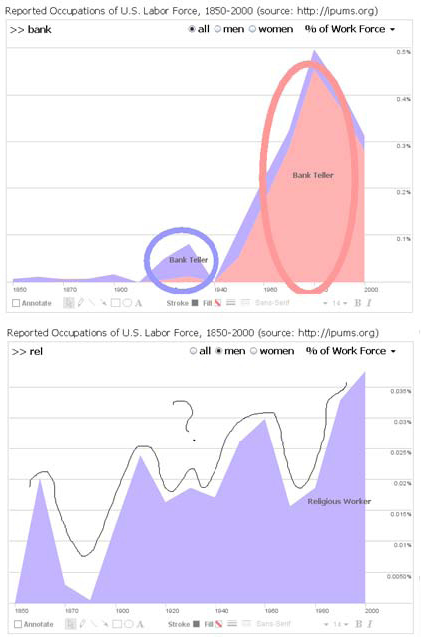
\includegraphics[height=0.7\columnwidth]{annotation-1}} 
\hfill
\subcaptionbox{Data-aware annotation.\label{fig:lr-annotation-2}}{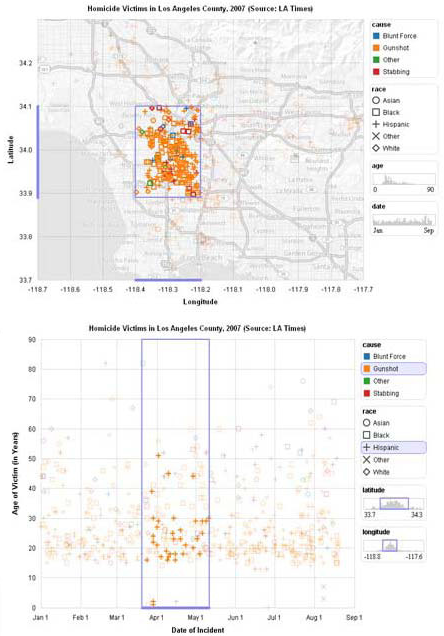
\includegraphics[height=0.7\columnwidth]{annotation-2}}
\caption{User annotation of bookmarked visualization.\is{Heer2012}}
\label{fig:lr-annotation}
\end{figure}

% Interaction
A note can simply be any user thought, but it can also take on different roles such as \emph{evidence}, \emph{assumption} and \emph{hypothesis}~\cite{Pike2009}. They have different visual representations, enabling users create and manage their complex reasoning processes. Typically, users are allowed to move notes freely and draw edges to connect them, enabling spatial grouping of related notes and relationships establishment. These interactive features are known to help users produce more critical thinking in their analyses~\cite{Sedig2013}. For example, users can show connections between a hypothesis and its evidence by drawing links, and spatially separate the evidence into a supporting group and a counter group, facilitating further comparison. \autoref{fig:lr-reasoning-simple-note} shows such a diagram produced with user notes and \autoref{fig:lr-reasoning-diagram-SRS} shows such a more formal diagram with different reasoning roles.

\begin{figure}[!htb]
\centering
\subcaptionbox{A diagram of user notes showing their thoughts. \is{Shrinivasan2008}\label{fig:lr-reasoning-simple-note}}{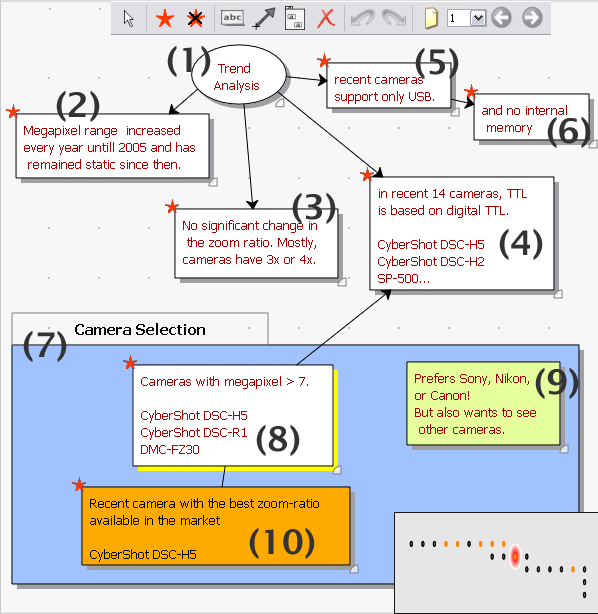
\includegraphics[height=0.42\columnwidth]{reasoning-simple-note}}
\hfill
\subcaptionbox{A formal reasoning diagram with nodes having different roles: evidence, casual relationship, assumption and hypothesis. \is{Pike2009a}\label{fig:lr-reasoning-diagram-SRS}}{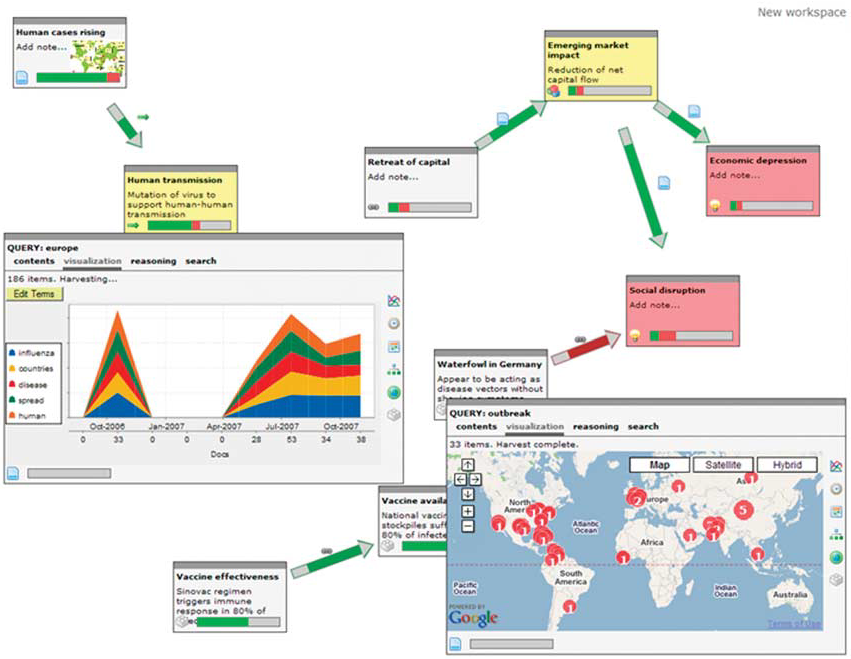
\includegraphics[height=.42\columnwidth]{reasoning-diagram-SRS}}
\caption{Visualization of reasoning process.}
\end{figure}

% Formal reasoning
More analytical reasoning methods have also been applied on the provenance data. The SRS system~\cite{Pike2009} first allows the user to construct a reasoning diagram with bookmarked visualizations as evidence nodes and causal relationships as links (\autoref{fig:lr-reasoning-diagram-SRS}). These evidence nodes and links may lead to a hypothesis. The user then specifies their confidence about the evidence before the system computes the likelihood of the hypothesis using the Dempster–Shafer belief network~\cite{Sanfilippo2007}. The result provides analytical support to the user. 

POLESTAR~\cite{Pioch2006} supports argument structuring, based on methods for analyzing legal documents such as the Toulmin model of argument~\cite{Toulmin2003}. To help validate a hypothesis, it organizes arguments as a tree structure of claims, each supported by at least one piece of evidence. A claim can have its supporting sub-claims and can also have rebuttals that weaken or restrict their force. \autoref{fig:lr-reasoning-argument-editor} shows such a argument tree. Sandbox~\cite{Wright2006} supports analysis of competing hypotheses -- a judgment method that requires careful weighing of alternative explanations~\cite{Heuer1999}. It allows users to add multiple hypotheses, each with supporting or contradictory evidence. These pieces evidence are weighted by the users and summarized in a visual matrix, enabling the users to effectively make a decision without having to remember and analyze in their minds. \autoref{fig:lr-reasoning-ACH} shows an example of this support.

\begin{figure}[!htb]
\centering
\subcaptionbox{Argument tree. Analysts elaborate arguments via a tree structure of claims, sub-claims, and facts. \is{Pioch2006}\label{fig:lr-reasoning-argument-editor}}{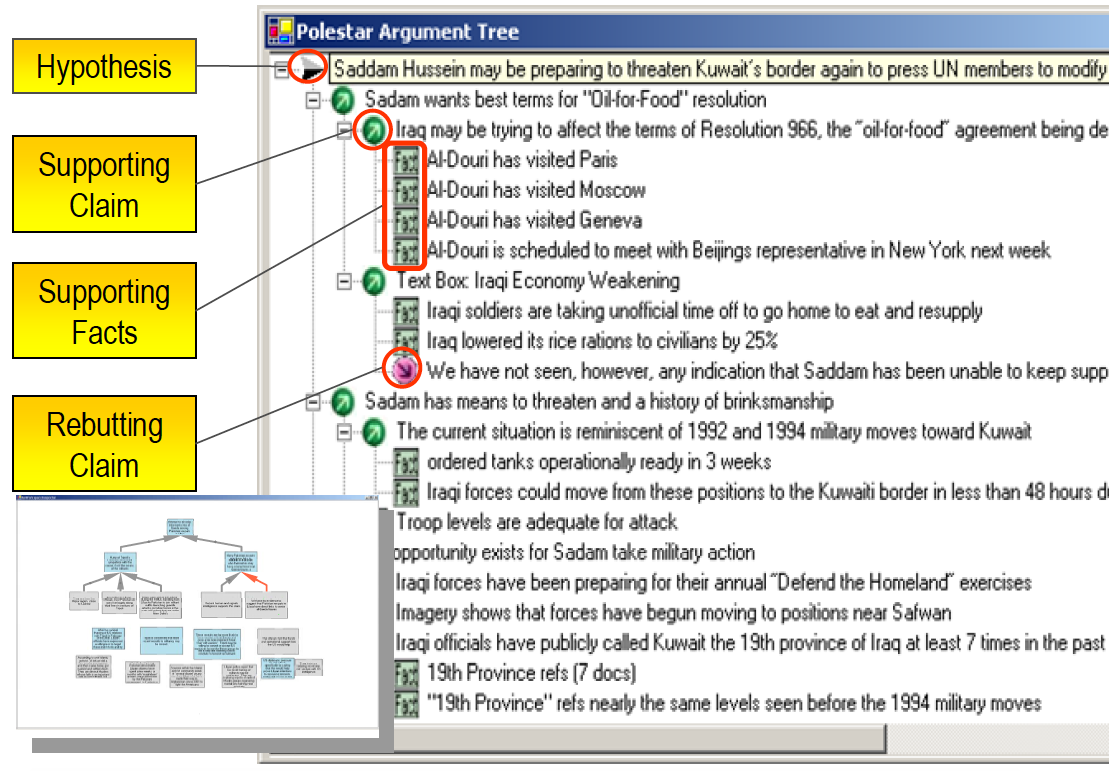
\includegraphics[height=0.3\columnwidth]{reasoning-argument-editor}}
\hfill
\subcaptionbox{Analysis of competing hypotheses. The interface allows adding multiple hypotheses, each with weighted supporting/counter evidence, and producing a summary matrix to evaluate them. \emph{\textrm{Image source: a video snapshot of~\cite{Wright2006}.}}\label{fig:lr-reasoning-ACH}}{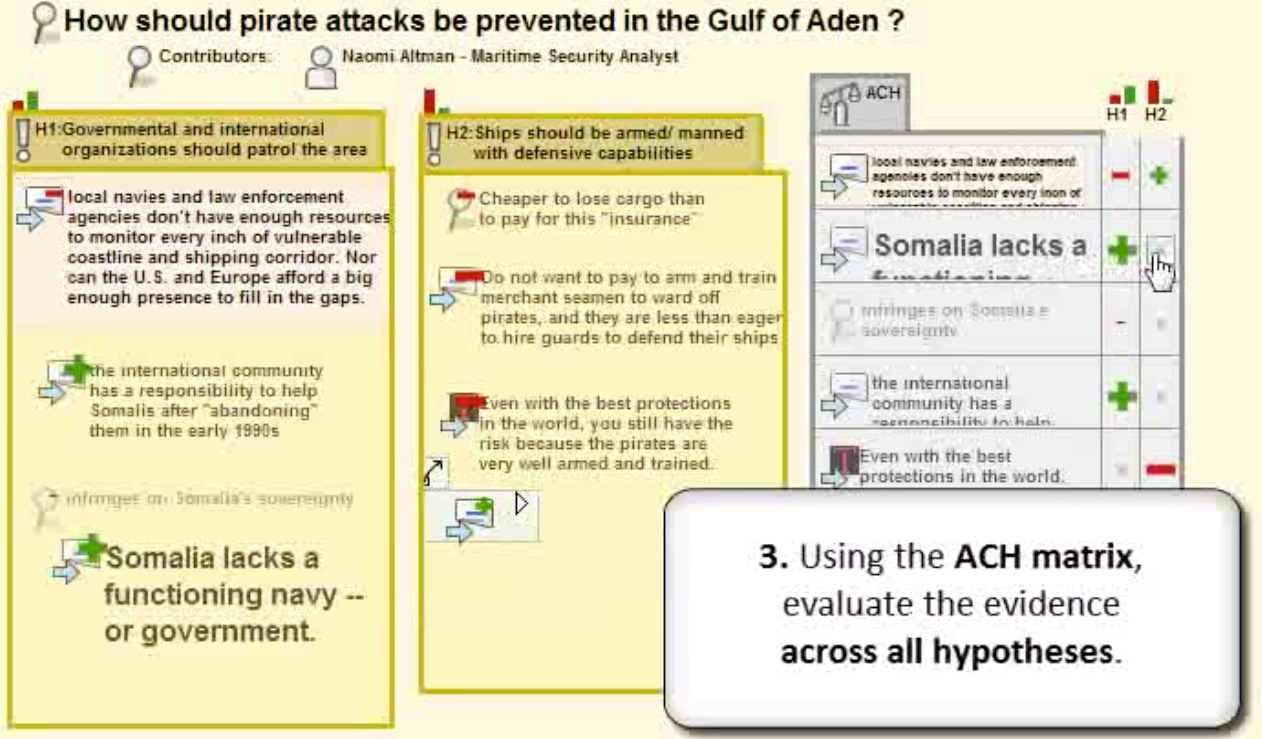
\includegraphics[height=0.3\columnwidth]{reasoning-ACH}}
\caption{Analytical support for the reasoning process.}
\label{fig:lr-reasoning}
\end{figure}
